\documentclass[12pt]{article}

\usepackage{sbc-template}

\usepackage{graphicx,url}

\usepackage[brazil]{babel}   
%\usepackage[latin1]{inputenc}  
\usepackage[utf8]{inputenc}  
% UTF-8 encoding is recommended by ShareLaTex

     
\sloppy

\title{Review: Performance Comparison of Mobile IPv4 and Mobile IPv6 Protocols in Wireless Systems}

\author{Antônio O. Junior\inst{1}, Cleverson V. Nahum\inst{1}, Felipe H. B. Bastos\inst{1}, Jamelly F. Ferreira\inst{1}, \\João C. Belmiro\inst{1} }


\address{Faculdade de Engenharia da Computação e Telecomunicações \\-- Universidade Federal do Pará
  (UFPA)\\
  Caixa Postal 479 -- 66.075-110 -- Belém -- PA -- Brazil
  \email{\{antonio,jamelly,felipe,joao\}@itec.ufpa.br, cleversonahum@ufpa.br}
}

\begin{document} 

\maketitle

\begin{abstract}
  In the last years, there has been a huge increase in the number of users connected in mobile networks, requesting better studies in this area. This review talk about this problem, comparing the MPIV4 model, more used in the
  moment, with the MIPV6 model that promises to improve the MIPV4 model, showing the qualities and the problems these   applications through the results results obtained in the article, Performance Comparison of Mobile IPv4 and
  Mobile IPv6 Protocols in Wireless Systems, R.Gunasundari and S.Shanmugavel.
\end{abstract}     
\begin{resumo} 
  Nos ultimos anos, ocorreu um enorme aumento no número de usuários conectados em redes móveis, solicitando melhores estudos nesta área. Esta resenha fala sobre este problema, comparando o modelo MPIV4, mais utilizado no momento, com o modelo MIPV6 que promete melhorar o modelo MIPV4, mostrando as qualidades e os problemas destas aplicações por meio dos resultados obtidos no artigo, Performance Comparison of Mobile IPv4 and Mobile IPv6 Protocols in Wireless Systems, R.Gunasundari and S.Shanmugavel.
\end{resumo}


\section{Introduction}

As already mentioned by many authors, the implementation the IPV6 protocol was necessary, mainly, because of the low addressing capacity of the IPV4 model.  Besides, the emergence the IPV6 protocol also contributed to IP mobility. However, what the objective the IP mobility? Basically, the mobility objective at the network layer is to allow that a device or node to move from one network to another, without changing your IP address, maintaining end to end communication of an application, one example is, the video stream, even if the device is on the move. 

The IETF (Internet Engineering Task Force) standardized Mobile IP in layers and IP mobility is already present in IPV4 protocol, but its use is not very efficient, because the delay and looses in the transfer of packages are very high.With this, the MIPV6 emerged to solve this problem, although it has not solved the high delay problem, it is more
effective that the MIPV4.

Coming up next, we present the article organization.  In chapter 2 we present the protocol overview, talking about MIPV4, MIPV6 and routing, while in chapter 3 we present the performance evaluation, where they are debated and questioned the simulations results. And finally, in chapters 4 and 5, we show our conclusions about the theme and this
article, and the studies references.

\section{Protocol Overview} \label{sec:firstpage}
%Parte João
\subsection{Mobile IPv4}

Users with MN (Mobile Node) have a local area network, and can move between different places, where an area is typically a remote network where the user connects to a wireless cell. Each of these areas has one or more FA (Foreign Agent), which are responsible for managing the permanence of MHs in their respective area, besides, each area has an HA (Home Agent), responsible for its local MNs, but who are visiting other areas.

Whenever an MN (Mobile Node) enters an area, it must register with the FA (Foreign Agent) responsible for this perimeter. The FA periodically broadcasts your address, announcing its presence for the new Mobile Nodes, which if they did not want to wait for the broadcast of the FA, they could also make a broadcast asking who the responsible FA is.

The mobile host registers with the FA, giving the address of its home agent and security information. The FA, in turn, contacts the HA (Home Agent), providing the safety information received from the MN, and announcing the presence of the MN in the area. Satisfied with the information, the HA informs AF to proceed with the registration, and the latter informs the MN that he is registered.

From this point, whenever a host tries to contact the MH, the packet addressed to it will be intercepted by the HA. On MN home network, because at first the sender does not know if the MH is in its permanent area or in another area. After intercepting the packet, the HA does the following: Encapsulates this packet in the data field of a new packet, and directs this new package to the FA responsible for the area where the MH is. This procedure is called tunneling. Notifies the sender of the original packet to send the next packets destined for the MH directly to the FA using the same tunneling technique. In this way, subsequent packets do not need to pass through HA.

MIPV4 presents a very innovative proposal regarding Internet access. However its implementation presents several problems to be overcome, Such as, the number of control messages to identify devices, improve the localization algorithm that is optimized in its successor MIPV6. In this way, it can be verified that the Mobile IP protocol presents deficiencies with respect to the scalability since as the number of devices increases, the protocol loses performance, this limits its use in new generation networks. Therefore, its use is impractical as it does not provide sufficient resources to meet current demands.

\subsection{Mobile IPv6}

MIPv6 (Mobile IPv6) is a protocol that was developed as a subset of Internet Protocol version 6 (IPv6) to support mobile connections. MIPv6 facilitates the movement of the node from one Ethernet type to another of the same type as well as the movement from an Ethernet network to a Wireless LAN cell.

MIPv6 is an update to the Mobile IP standard (RFC 2002), created by the Internet Engineering Task Force (IETF), and is designed to authenticate mobile devices (known as mobile nodes) using IPv6 addresses. Mobile IPv6, like MIP, allows a mobile node to move from one network to another without breaking a connection. This means that the original address(home address) never changes, the mobile node (MN) can be anywhere, that the packets will be routed correctly to it through appropriate mechanisms Motion is thus transparent to the transport layer and to applications that use the TCP IP and Mobile IPv6 protocol.

The home address is made up of a valid prefix in the link of your home network. It is through this address that a corresponding node will communicate with the mobile node, regardless of where it is. When the mobile node changes its network, it maintains the home address and receives another address, the care-of address (COA), consisting of a valid prefix on a foreign network. This address is acquired stateless or stateful, (without or with address server, 
respectively). In this way, MN will have a home address and one or more care-of address when it is moving between networks. In order to be able to know where the mobile node is, an association between home address and care-of address must be performed (binding). This care-of address is made by the mobile node, in the home agent (HA). This association is performed through a binding registration, where the MN sends messages called Binding Updates (BU) to the HA, which responds with a Binding Acknowledgment (BA) message.

The corresponding nodes (CNs) in IPv6 have "intelligence" for route optimization, that is, they can store bindings between home address and care-of-address of mobile nodes. Thus, a mobile node can provide information about its location for CNs, through the corresponding binding procedure. In this procedure, a binding establishment authorization mechanism is performed, called the return routability procedure. Note that the Foreign Agent (FA), present in MIPv4, no longer exists. Communication between MN and CN can take place in two ways:

  Bidirectional tunneling: does not require that the CN has MIPv6 support and that the MN has registered with the CN. The packets are routed from the CN to the HA and the HA is tunneled to the MN. Then the MN responds to the HA by tunnel which, in turn, responds to the CN. Each intercepted packet is tunneled for MN's care-of address.

Route optimization: the CN must support MIPv6 ("intelligence" for binding) and the MN must register with the CN. In this case, the CN, before sending the packet, searches in a cache for an association between home address and care-of address of MN. If there is an association, the packet will be routed to the care-of address of the mobile node directly. This eliminates congestion in the home link and in HA. The MIPV6 protocol corrects several of its predecessor's failures, increasing the quality of the protocol as a whole, increasing the chances of being implemented on a large scale, being able to offer free Internet to mobile devices, and compete with the telephone operators that offer 3G and 4G Internet services in Brazil. However the standardization for the IPv6 protocol follows slowly for home users, as the price of the equipment is not affordable, regarding security the IPV6 itself offers parts in its headers to insert security algorithms that IPv4 does not offer, however there is still the use of unidentified binding updates, which are treated as a security problem, as this feature allows packets destined To a mobile host being sent to a remote address (COA), unauthenticated use of it could lead to malicious updates that would lead a correspondent to send packets destined for the mobile host to a third host. There is still the scalability problem of its previous version that does not allow the connection of multiple mobile nodes on a single network. But there is still the possibility of applying the mobility in our daily life because the Internet is 
increasingly more collaborative.


% Cleverson's Session
\subsection{Main changes of MIPv4 to MIPv6}
The author talk about main differences between MIPv4 and MIPv6, he quote the address configuration, route optimization, routing header and ingress filter bypass. With IPv6, the address configuration in the network does not need more of NAT, because it has more address for to assign, with this the network does not has need to do the translation between a global address for a local address, thus it does not need to has a foreign agent. Furthermore, with IPv6 each interface has a certain address received of sub network, it is important, because its facilitate the work of DHCPv6 for to set addresses for nodes, this addresses are unique.

In MIPv4 all the packets pass through the home network, after this, the packets will forward to foreign network until to be transmitted for the mobile node, this process is named like triangular routing. All the times in one connection the packets will do this path in MIPv4, but with MIPv6 we have a route optimization, in its just the first packet need to pass though home network, after this first time the mobile node will send a binding update to the correspondent node with its care of address of its, thus the correspondent node can to transmit packets directly for the mobile node in the next transmission of packet. With this changes the MIPv6 solved problems with triangular routing and improvement the efficiency of transmission.

For to do transmissions in MIPv4 we need to pass packet of correspondent node to home agent, in there the packet is involved into a other packet IP with the care of address, this process is named like IP-within-IP. The MIPv6 uses other approach, the care of address is inserted in a value in header of IPv6, with this is possible to define for where the packets to be forwarding until to come to mobile node. This process adopted by MIPv6 use less bytes than process of MIPv4 (IP-Within-IP) thus reducing the overhead of packet delivery.

In MIPv6, it is possible to use both the transmission through Home Address like in MIPv4 or a direct transmission for to care-of-address after the first transmission through Home Address, because after this it is possible to know the care-of-address of mobile node. Sometimes, the network has a high delay in a link due a congestion, so it is important to have more option for to do transmission for a mobile node, this process is named ingress filter bypass. With this, it can to do a balance between the links contributing for a better distribution in the transmissions in the network.

So, the design of MIP actual is a improvement gained with all the experiences lived with MIPv4 and now with MIPv6. MIPv4 had many problems and with the MIPv6 many problems of it was solved, some functions was improvement into MIPv6 and new functionalities were added.


\section{Performance Evaluation}

%jamelly's part
\subsection{Simulations analisys}
In the article some features are explored in order to show the behavior of both MIPv6 and MIPv4 in wireless networks. All the simulation is done with ns-2 in the version 2.1b6 and in the implementation of MIPv4 the DSDV was kind of implemented with 	Mobiwan Module. The approach used in the article is based in a situation where there is one single MN moving between HA and FA(as showed in figure 1). Finally, the analyzed features are : 
\begin{enumerate}
\item Throughput of receiving bits Variation with Average Simulation End to End Delays
\item Variation of packet Id with Simulation End to End Delay
\item TCP traffic affected by Router Solicitation
\end{enumerate} 

%pay attemption to this figure

\begin{figure}[ht]
\centering
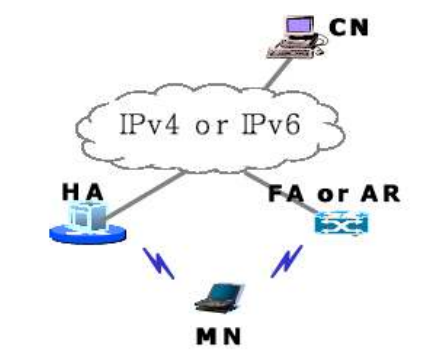
\includegraphics[width=.3\textwidth]{simulation_approach.png}
\caption{The approach used in the simulation.}
\label{fig:simulation_approach}
\end{figure}


\subsubsection{Throughput of receiving bits Variation with Average Simulation End to End Delays}

Before getting started, it is needed to explain what is End to End delay. The End to End delay is \textit{the sum of all the delays got in each node that the packet pass through}. In the article is easily perceptible the almost linear relation between the characteristics observed. Using the figures 2 and 3 is perceptible too that the delay starts to increase from 1200Kbytes from both MIPv4 and MIPv6. There is a considerable number of similarities but the differences start when in MIPv4 the delay decreases with a throughput of 2800Kbytes while in MIPv6 it still increases with a single detail : the delay in MIPv6 is less compared to MIPv4.

\begin{figure}[ht]
\centering
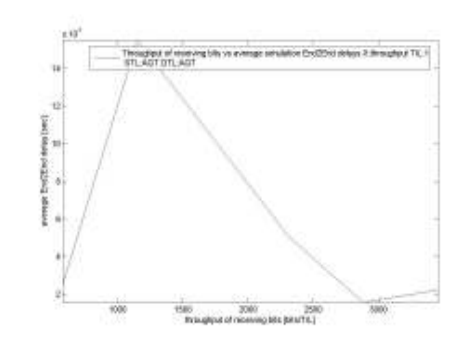
\includegraphics[width=.3\textwidth]{topico1_mipv4.png}
\caption{Throughput of receiving bits Variation with Average Simulation End to End Delays in MIPv4}
\label{fig:topico1_mipv4}
\end{figure}


\begin{figure}[ht]
\centering
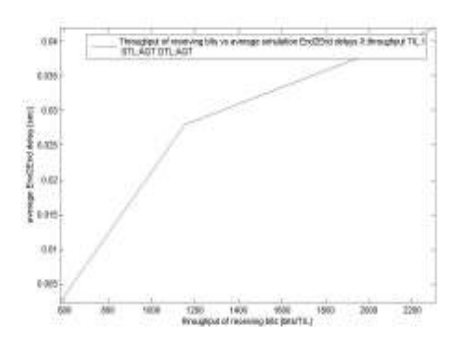
\includegraphics[width=.3\textwidth]{topico1_mipv6.png}
\caption{Throughput of receiving bits Variation with Average Simulation End to End Delays in MIPv6.}
\label{fig:topico1_mipv6}
\end{figure}
  


\subsubsection{Variation of packet Id with Simulation End to End Delay}
Other important aspect in the analysis, this aspect bring a important information about the protocols. It is possible to percept that in MIPv6 the delay is lower, it happens mainly because in MIPv4 the total amount of transmitted package is considerable higher than in MIPv6, what increases the probability of disconnection what makes the cost of the handover take high values.

\begin{figure}[ht]
\centering
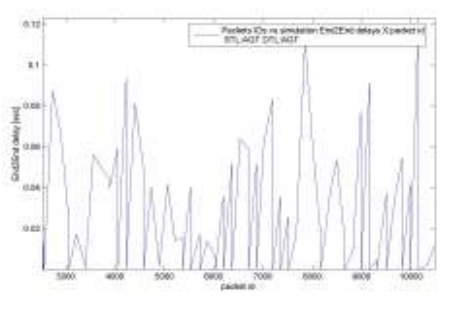
\includegraphics[width=.3\textwidth]{topico2_mipv4.png}
\caption{Variation of packet Id with Simulation End to End Delay for MIPv4.}
\label{fig:topico2_mipv4}
\end{figure}


\begin{figure}[ht]
\centering
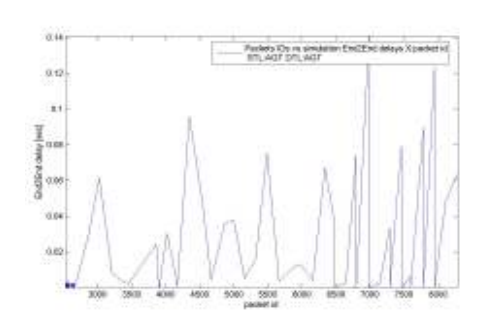
\includegraphics[width=.3\textwidth]{topico2_mipv6.png}
\caption{Variation of packet Id with Simulation End to End Delay for MIPv6.}
\label{fig:topico2_mipv6}
\end{figure}



\subsubsection{TCP traffic affected by Router Solicitation}

In the Mobile Ip protocols, the process of registration is a pretty important step that has a important participation of advertisements from the router, losing these can make the registration time out. In MIPv4 there's a big problem cause it offers a small time of registration, what causes a great possibility to lose the advertisements from the router, and in consequence of that lose the registration process. In MIPv6 this problem is softer cause its long registration period don't compromise the registration process, the only cause to lose performance is when the MN is out of the basestation coverage and it is solved with IPV6 extensions. The figures show us situations where the MN doesn't receives advertisements neither from MH or FH, and we can percept that in a certain period that the performance is very damaged, that's the registration time.

\begin{figure}[ht]
\centering
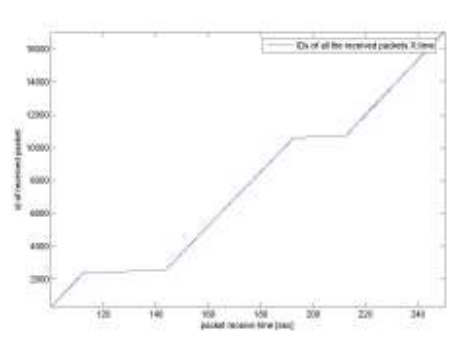
\includegraphics[width=.3\textwidth]{topico3_mipv4.png}
\caption{TCP traffic affected by Router Solicitation for MIPv4.}
\label{fig:topico2_mipv4}
\end{figure}


\begin{figure}[ht]
\centering
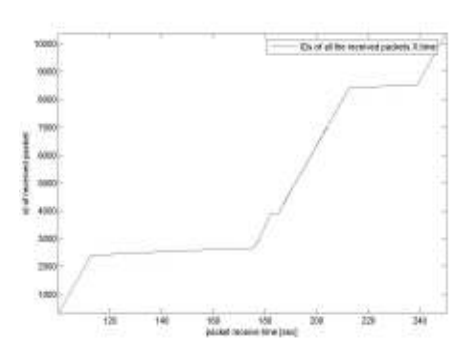
\includegraphics[width=.3\textwidth]{topico3_mipv6.png}
\caption{TCP traffic affected by Router Solicitation for MIPv6.}
\label{fig:topico2_mipv6}
\end{figure}


\section{Conclusion}

The MIPv4 and MIPv6 were solution very important for its times, but nowadays much concepts about networks and the needs of people changed. With this the network need to change together, because this we have discussed about the future Internet and new architectures.



\section{References}
Gunasundari R and Shanmugavel S, 'Performance Comparison of Mobile IPv4 and Mobile IPv6 Protocols in Wireless Systems', IEEE, 2009.

Johnson D, Perkins C and Arkko.J,’Mobility support in IPv6', IETF RFC 3775, 2004.

Thomson.S and T.Narten, ‘IPv6 stateless address auto configuration’, IETF  RFC 1971, 1996.


\bibliographystyle{sbc}
\bibliography{sbc-template}

\end{document}